\chapter{Methods}
\label{ch:methods}

\section{Constant Velocity Path Following (Unicyclic)}

As a base method to improve on, a Nonlinear Path Following Guidance\cite{stastny_flying_2019} for a Fixed Wing vehicle was chosen because the Fixed Wing presents the most conservative and constrained platform, and thus can be extended easily to incorporate a more agile platform (e.g. Multirotor).\\

Since Fixed Wing has a relatively constant forward speed, the algorithm thus assumes a 'unicyclic' motion, as if the vehicle was a person riding a unicycle with a constant speed. This means that only the direction of travel may change (heading), and not its speed.

\begin{figure}[h]
\centering
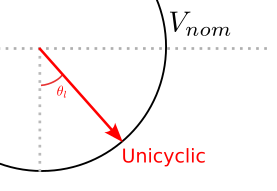
\includegraphics[width=0.7\textwidth]{Unicyclic_Formulation}
\caption{Unicyclic Formulation}
\label{fig:unicyclic_formulation}
\end{figure}

Here first the track error boundary gets defined proportional to the nominal speed $V_{nom}$. This is to make the path following magnitude independent and thus have a fixed convergence time. And the time constant $\tau_{const}$ can be set by the user, which in turn will define the acceleration that occurs when following the vector field.

\begin{equation}
    e_b = V_{nom} \cdot \tau_{const}
\label{eq:unicyclic_track_error_boundary}
\end{equation}

Here the look ahead angle $\theta_l$ is defined by the normalized track error $\overline{e}$, as in \cite{stastny_low-altitude_2020} defined in \autoref{eq:unicyclic_quadratic_laa_curve}.

\begin{equation}
    \theta_l = \frac{\pi}{2}(1-\overline{e})^2
\label{eq:unicyclic_quadratic_laa_curve}
\end{equation}

As shown in \autoref{fig:unicyclic_formulation}, when a desired course angle ($\theta_l$, relative to $\hat{t_p}$) is given, the desired ground velocity in the absence of wind essentially becomes $V_ref(e) = V_{nom} \cdot \hat{l}(e)$, where $\hat{l}$ is the unit vector pointing in the direction of a desired course angle.\\

This leads to the final reference velocity calculation like following

\begin{equation}
    \begin{split}
        V_{ref}^{\perp} &= V_{nom} \cdot cos(\theta_l)\\
        V_{ref}^{\parallel} &= V_{nom} \cdot sin(\theta_l)
    \end{split}
\label{eq:hybrid_velocity_components}
\end{equation}

Then (in the original formulation $V_{nom}$ is ignored in the absence of wind, and only heading error gets calculated) the heading error proportionally commands a lateral acceleration, which brings the vehicle on its desired heading, achieving the desired course angle.\\

Therefore the estimation of the vehicle's heading is a crucial factor in this formulation, which is why it isn't ideal for multirotor use cases since it doesn't have an acceleration capability tied to the heading.

\section{Variable Velocity Path Following (Hybrid)}

To overcome the aforementioned limitation of the Unicyclic formulation, a new 'Hybrid' formulation is presented. It is essentially an adaptation of the Unicyclic formulation to account for a flexible velocity range  of a Multirotor and a different meaning behind the vector field itself.

\begin{figure}[h]
\centering
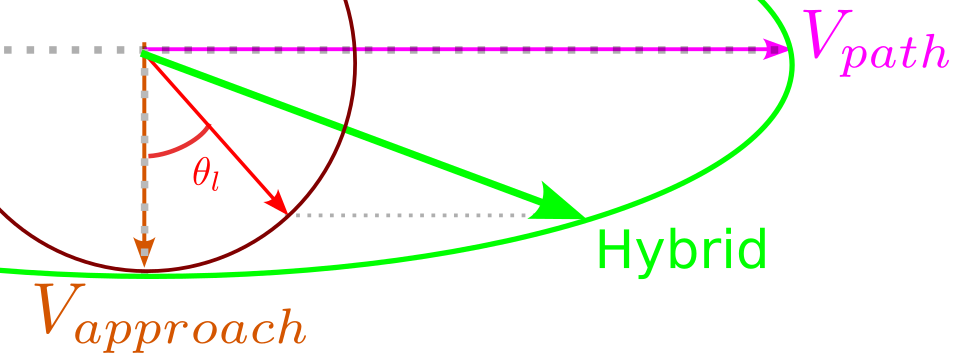
\includegraphics[width=0.7\textwidth]{Hybrid_Formulation}
\caption{Hybrid Formulation}
\end{figure}

Unlike the unicyclic method, hybrid has a variable $V_{path}$ component parallel to path, and $V_{approach}$ component orthogonal to path. And it is essentially an ellipse that is stretched in each axis to match the approach \& on-path constraints described in \autoref{seq:approach_on_path_vel_constraints}.

Track error boundary gets defined very similarly to the Unicyclic case, proportional to the approach speed $V_{approach}$. This was done because the convergence time depends on the orthogonal velocity curve. And the time constant $\tau_{const}$ can be set by the user, which in turn will define the acceleration that occurs when following the vector field.

\begin{equation}
    e_b = V_{approach} \cdot \tau_{const}
\label{eq:hybrid_track_error_boundary}
\end{equation}

Here the look ahead angle $\theta_l$ is defined by the normalized track error $\overline{e}$, as in \cite{stastny_low-altitude_2020} defined in \autoref{eq:hybrid_quadratic_laa_curve}.

\begin{equation}
    \theta_l = \frac{\pi}{2}(1-\overline{e})^2
\label{eq:hybrid_quadratic_laa_curve}
\end{equation}

This leads to the final reference velocity calculation like following

\begin{equation}
    \begin{split}
        V_{ref}^{\perp} &= V_{approach} \cdot cos(\theta_l)\\
        V_{ref}^{\parallel} &= V_{path} \cdot sin(\theta_l)
    \end{split}
\label{eq:hybrid_velocity_components}
\end{equation}

Along with it, the interpretation of the Velocity vector field is not just in terms of the desired course angle, but actually incorporates the exact velocity vector vehicle would need to achieve as shown in \autoref{fig:mc_fw_vector_field_pipeline}.

\begin{figure}[h]
\centering
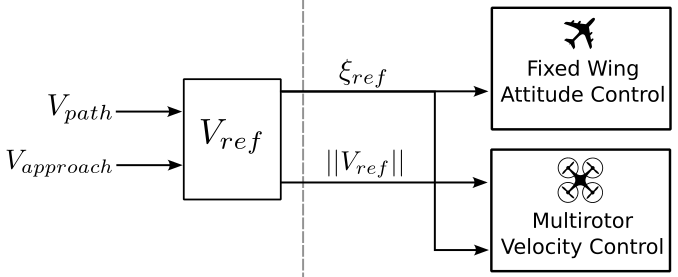
\includegraphics[width=0.7\textwidth]{VF_MC_FW_Pipeline}
\caption{Multirotor and Fixedwing control pipeline from the Vector Field}
\label{fig:mc_fw_vector_field_pipeline}
\end{figure}

This is possible because a multirotor can follow any velocity setpoint in any condition/heading. Furthermore, it doesn't get affected as much as in fixed wing case, so we can assume that any sane velocity setpoint within the vehicle's capability is feasible.\\

Notice how only the desired heading $\xi_{ref}$ is taken for fixed wing attitude control, and for multirotor the full velocity vector $V_{ref}$ is taken as an input.